\documentclass[12pt,a4paper]{report}
\usepackage[utf8]{inputenc}
\usepackage[T1]{fontenc}
\usepackage[brazil]{babel}
\usepackage[a4paper,margin=2.5cm]{geometry}
\usepackage{graphicx}
\usepackage{booktabs}
\usepackage{amsmath}
\usepackage{float}
\usepackage[round,authoryear]{natbib}
\usepackage[hidelinks]{hyperref}
\graphicspath{{../outputs/figures/}}
\setlength{\parskip}{0.4em}
\renewcommand{\arraystretch}{1.15}

\begin{document}

% ----------------------------------------------------------------- CAPA
\begin{titlepage}
\centering
\vspace*{1cm}
{\scshape\large Fundação Getulio Vargas \\ Escola de Economia de São Paulo (EESP)\par}
\vspace{2.5cm}
{\huge\bfseries Forecasting da exposição de gestoras de ações\par}
\vspace{0.8cm}
{\Large Medição da exposição (R\$/US\$), previsibilidade da demanda e extensão exploratória sobre estruturas fundo-sobre-fundo --- evidência do mercado brasileiro de fundos, 2016--2021\par}
\vspace{3cm}
{\Large João Paulo Zangrandi\par}
\vspace{0.5cm}
{\large Orientador: Prof.\ Maurício Ferraresi Junior\par}
\vfill
{\large São Paulo \\ \today\par}
\end{titlepage}

% --------------------------------------------------------------- RESUMO
\chapter*{Resumo}
\addcontentsline{toc}{chapter}{Resumo}
Este trabalho mede a exposição das gestoras brasileiras a ações e testa sua previsibilidade sob a ótica do
\emph{demand-based asset pricing} \citep{koijenyogo2019,gabaixkoijen2021}. O \textbf{núcleo empírico} usa as
bases públicas da CVM originalmente selecionadas para o projeto --- composição consolidada de carteiras
(CONS) e série histórica (SH) --- para construir um \emph{pipeline} reprodutível em R que mede a exposição em
\textbf{valor} (R\$ e US\$), na definição \emph{net}, consolidando grupos econômicos e mantendo os FICs.
Três resultados principais: (i)~um painel gestora $\times$ mês $\times$ ação validado contra os dados reais
(ITUB4 e 836 ações, 2016--2021); (ii)~uma avaliação \emph{out-of-sample} mostrando que a \emph{variação}
mensal da exposição é essencialmente imprevisível (martingale), ao passo que o \emph{nível} reverte à média
de forma previsível ($\sim$10\% sobre o \emph{random walk}) apenas nas \emph{blue chips} mais concentradas; e
(iii)~uma extensão \textbf{exploratória} com a base não consolidada de cotas de fundos (CDA, Bloco~2), que
reconstrói relações fundo$\to$fundo e sugere dupla contagem interna relevante (FIC$+$master da mesma gestora,
$\approx 37\%$). Como a CDA não faz parte do desenho inicial validado com o orientador, seus resultados são
tratados como evidência complementar e devem ser confirmados antes de se tornarem o eixo central do TCC. As
ações mais ``concentradas'' (detidas por todas as gestoras) são as mesmas mais frágeis no sentido de
\citet{greenwoodthesmar2011}.

\noindent\textbf{Palavras-chave:} demand-based asset pricing; exposição em ações; previsibilidade; fundos de
cotas; CVM.

\tableofcontents

% =================================================================
\chapter{Introdução}\label{cap:intro}
O objetivo central deste trabalho é medir e testar a previsibilidade da \textbf{exposição das gestoras a
ações}. O método é validado com uma ação (ITUB4, Itaú Unibanco PN) e depois estendido a todas as ações
identificáveis nas carteiras. Uma dimensão adicional é que parte dessa exposição passa por fundos de cotas
(FIC), o que pode criar participações sobre participações; essa dimensão, porém, é tratada aqui como uma
\textbf{extensão exploratória} baseada na CDA, não como premissa necessária para o painel principal.

A motivação teórica é o \emph{demand-based asset pricing}: \citet{koijenyogo2019} formalizam a formação de
preços pela demanda dos investidores institucionais, e \citet{gabaixkoijen2021} mostram que o mercado é
inelástico, de modo que fluxos têm impacto desproporcional. Se a demanda das gestoras tem estrutura, ela é
em parte previsível e pode se propagar; \citet{greenwoodthesmar2011} ligam a sobreposição de propriedade à
\emph{fragilidade de preços}. Daí três perguntas: \textbf{(1)} é possível medir corretamente a exposição em
valor com CONS e SH? \textbf{(2)} a exposição é previsível? \textbf{(3)} como extensão, a rede
fundo-sobre-fundo observável na CDA altera a leitura de duplicação e risco?

\paragraph{Contribuições.} (i)~Pipeline validado de exposição (R\$/US\$, net, grupos, FICs) para ITUB4 e
836 ações usando CONS+SH; (ii)~avaliação \emph{out-of-sample} da previsibilidade da exposição; (iii)~módulo
exploratório de grafo fundo-sobre-fundo (CDA Bloco~2) e quantificação da dupla contagem interna
($\approx 37\%$) quando essa base adicional é incorporada.

% =================================================================
\chapter{Revisão bibliográfica}\label{cap:rev}
\textbf{Demand-based asset pricing.} \citet{koijenyogo2019} estimam um sistema de demanda a partir de
carteiras institucionais; \citet{gabaixkoijen2021} quantificam a baixa elasticidade do mercado agregado.
\textbf{Propriedade comum e fragilidade.} \citet{greenwoodthesmar2011} introduzem medidas de fragilidade
baseadas na concentração e correlação da propriedade --- diretamente aplicáveis à sobreposição de carteiras.
\textbf{Métodos.} Fatores latentes via PCA/análise fatorial seguem \citet[cap.\ 3--4]{artesbarroso2023}; no
módulo exploratório com CDA, a rede de fundos como grafo remete a \citet{sanchezlengeling2021}.
\textbf{Plataformas.} A referência central do orientador é \emph{Replicant Investment Platforms}
\citep{ferraresi_replicant}, que trata plataformas (vasos que investem entre gestoras) como unidade de
análise. Essa ponte teórica é relevante para a extensão com CDA, mas a citação bibliográfica exata e o papel
desse eixo devem ser confirmados com o orientador.

% =================================================================
\chapter{Dados}\label{cap:dados}
Duas bases públicas da CVM formam o núcleo do trabalho (CONS e SH, 2016--2021, separador ``\texttt{;}'').
A CDA é usada apenas em um módulo complementar para estudar relações fundo$\to$fundo.

\paragraph{CONS --- composição consolidada (\emph{holdings}).} Granularidade fundo $\times$ mês $\times$
ativo ($\sim$21,1 milhões de linhas). Valores em \textbf{formato americano} (ponto decimal); a base é
\textbf{100\% ``Ações''} --- a consolidação da CVM dissolve as cotas em ações. Três variantes por ticker:
direta, cedida em empréstimo e obrigações (aluguel tomado, negativa). Cobertura de \emph{ticker}: $\sim$99\%
($\sim$1\% são ações de companhia fechada, sem código).

\paragraph{SH --- série histórica.} Granularidade fundo $\times$ dia; traz a \textbf{gestora} e o \textbf{PL}.
Formato brasileiro (\texttt{R\$ 49.749,57}). 50 gestoras e 52,6\% de linhas FIC em 2016.

\paragraph{CDA --- Bloco~2 (cotas de fundos), não consolidada; extensão exploratória.} A CDA preserva
relações fundo$\to$fundo que a CONS apaga: cada linha é ``A detém cotas de B'' (\texttt{CNPJ\_FUNDO},
\texttt{CNPJ\_FUNDO\_COTA}, \texttt{VL\_MERC\_POS\_FINAL}). Extraímos \textbf{835.694 arestas} com origem nos
fundos da amostra. Como essa base não fazia parte do desenho inicial do projeto, seus resultados são
mantidos separados do núcleo CONS+SH até validação explícita com o orientador.

\paragraph{Ligação.} \texttt{Código} (CONS) $=$ \texttt{COD\_FUNDO} (SH) por CNPJ (verificado: apenas 2
fundos-mês da CONS sem correspondência no SH; \emph{overlap} de CNPJ $\approx 100\%$).

\section{Revisão de qualidade das bases}\label{sec:qualidade}
Auditamos cada afirmação contra os dados reais (Tabela~\ref{tab:qual}). Destaques: a CONS é 100\% ``Ações''
em todos os anos e os valores estão de fato em formato americano (uma versão anterior do painel estava
corrompida por um erro de \emph{parsing} que removia o ponto decimal --- corrigido). Encontramos $\sim$0,2\%
de \textbf{linhas exatamente duplicadas} (mesmo fundo/data/ativo/valor; artefatos de exportação), que
deduplicamos --- impacto de $\approx 0{,}01\%$ nos totais. No SH, \emph{nenhum} CNPJ tem mais de uma classe
e \emph{nenhum} fundo troca de gestora, o que valida a consolidação por grupo e afasta dupla contagem de PL.
Dos fundos do SH sem carteira na CONS (cobertura média 74,8\%), \textbf{94,7\% não são fundos de ações}
(renda fixa/multimercado) --- ausência esperada. Na CDA, a fração de propriedade
$\phi=\text{valor}/PL_{\text{destino}}$ tem mediana próxima de 0,007 e fica em $(0,1]$ em aproximadamente
98,6\% dos casos, validando as unidades em primeira ordem; não há \emph{self-loops}. O campo
\texttt{DT\_CONFID\_APLIC} aparece preenchido em parte das arestas, mas nos arquivos históricos processados
o \texttt{CNPJ\_FUNDO\_COTA} está disponível; portanto, ele não deve ser descrito como destino mascarado sem
checagem adicional.

\begin{table}[H]\centering
\caption{Revisão das bases (2016--2021): fato e resultado.}
\label{tab:qual}
\small
\begin{tabular}{ll}
\toprule
\textbf{Verificação} & \textbf{Resultado} \\
\midrule
CONS 100\% ``Ações''                 & sim, todos os anos \\
Magnitudes 2016 (net ITUB4)          & direta R\$\,35,4 bi; cedida R\$\,9,6 bi; obrig.\ $-$R\$\,5,8 bi \\
Linhas exatamente duplicadas         & $\sim$0,2\% (deduplicadas; impacto $\approx$0,01\%) \\
SH: classes por CNPJ / troca gestora & 1 / 0 (sem dupla contagem de PL; grupos estáveis) \\
Cobertura SH em CONS                 & 74,8\%; 94,7\% dos ausentes não são de ações \\
Chave Código $=$ COD\_FUNDO          & sim (2 fundos-mês sem match) \\
CDA: $\phi$ (propriedade)            & mediana $\approx$0,007; 98,6\% em $(0,1]$; 0 \emph{self-loops} \\
CDA: escopo                          & extensão exploratória; destinos externos existem; confidencialidade requer leitura cautelosa \\
\bottomrule
\end{tabular}
\end{table}

% =================================================================
\chapter{Metodologia}\label{cap:metodo}
\textbf{Unidade:} gestora, consolidada por grupo econômico (Itaú, BTG, XP\ldots), via regex sobre o nome
normalizado. \textbf{Medida:} valor (não quantidade), em R\$ e US\$ (PTAX fim de mês, BCB SGS série~1).
\textbf{Exposição:} três definições, geradas em paralelo --- \texttt{direta} (só a linha direta),
\texttt{long} ($+$cedida) e \texttt{net} ($+$obrigações); a primária é a \emph{net}. \textbf{FICs mantidos}
no painel principal, porque são fundos reais da amostra; eventual dupla contagem é tratada apenas no módulo
exploratório com CDA. \textbf{Estacionariedade:} modela-se a posição (não-estacionária $\to$
diferenciar) e seu nível; o peso é descritivo; ADF reportado.

\paragraph{Módulo exploratório: grafo fundo-sobre-fundo.} Nó $=$ fundo; aresta direcionada ``detém cotas de''
(CDA), ponderada pelo valor. Métricas: detecção de ciclos, profundidade de aninhamento e
\textbf{look-through de-duplicado}. Esta etapa não é necessária para construir o painel de exposição e deve
ser entendida como extensão metodológica.

\paragraph{De-duplicação.} Somar a exposição entre fundos da mesma gestora dupla-conta: se A detém a fração
$\phi_{A\to B}=v_{A\to B}/PL_B$ de B, a exposição consolidada de A já inclui $\phi_{A\to B}L_B$, que também
está em $L_B$. Logo
\[ \text{dedup}_g = \sum_{i\in g} L_i - \!\!\sum_{A\to B\,\in g}\!\! \phi_{A\to B}\,L_B . \]

\paragraph{Forecasting.} Avaliação \emph{out-of-sample} com origem móvel (janela expansível), 1 passo, sem
vazamento, contra o \emph{random walk}; métricas RMSE/MAE (\emph{skill} vs RW) e acerto de direção.

% =================================================================
\chapter{Resultados}\label{cap:result}

\section{Exposição das gestoras}\label{sec:exp}
O painel (ITUB4) tem 2.835 observações gestora-mês (42 grupos, 72 meses); o peso varia entre $-6\%$ e
$+21\%$ (mediana 0,84\%). As maiores posições são de Itaú ($\sim$US\$\,500 mi médios), Bradesco, BB,
Kapitalo e Santander (Figura~\ref{fig:pos}). A Tabela~\ref{tab:expo} compara as definições: a soma das
posições mensais vai de R\$\,468 bi (direta) a R\$\,540 bi (long) e R\$\,496 bi (net); sob a net, 264 das
2.835 observações ficam \emph{net short} (aluguel $>$ posição), o que nunca ocorre nas demais.

\begin{table}[H]\centering
\caption{Definições de exposição (ITUB4): soma das posições mensais e \emph{net short}.}
\label{tab:expo}
\small
\begin{tabular}{lrrr}
\toprule
\textbf{Definição} & \textbf{Soma (R\$ bi)} & \textbf{Pos.\ média (US\$ mi)} & \textbf{Obs.\ net short} \\
\midrule
direta & 468 & 39,0 & 0 \\
long   & 540 & 45,1 & 0 \\
net    & 496 & 41,4 & 264 \\
\bottomrule
\end{tabular}
\end{table}

\begin{figure}[H]\centering
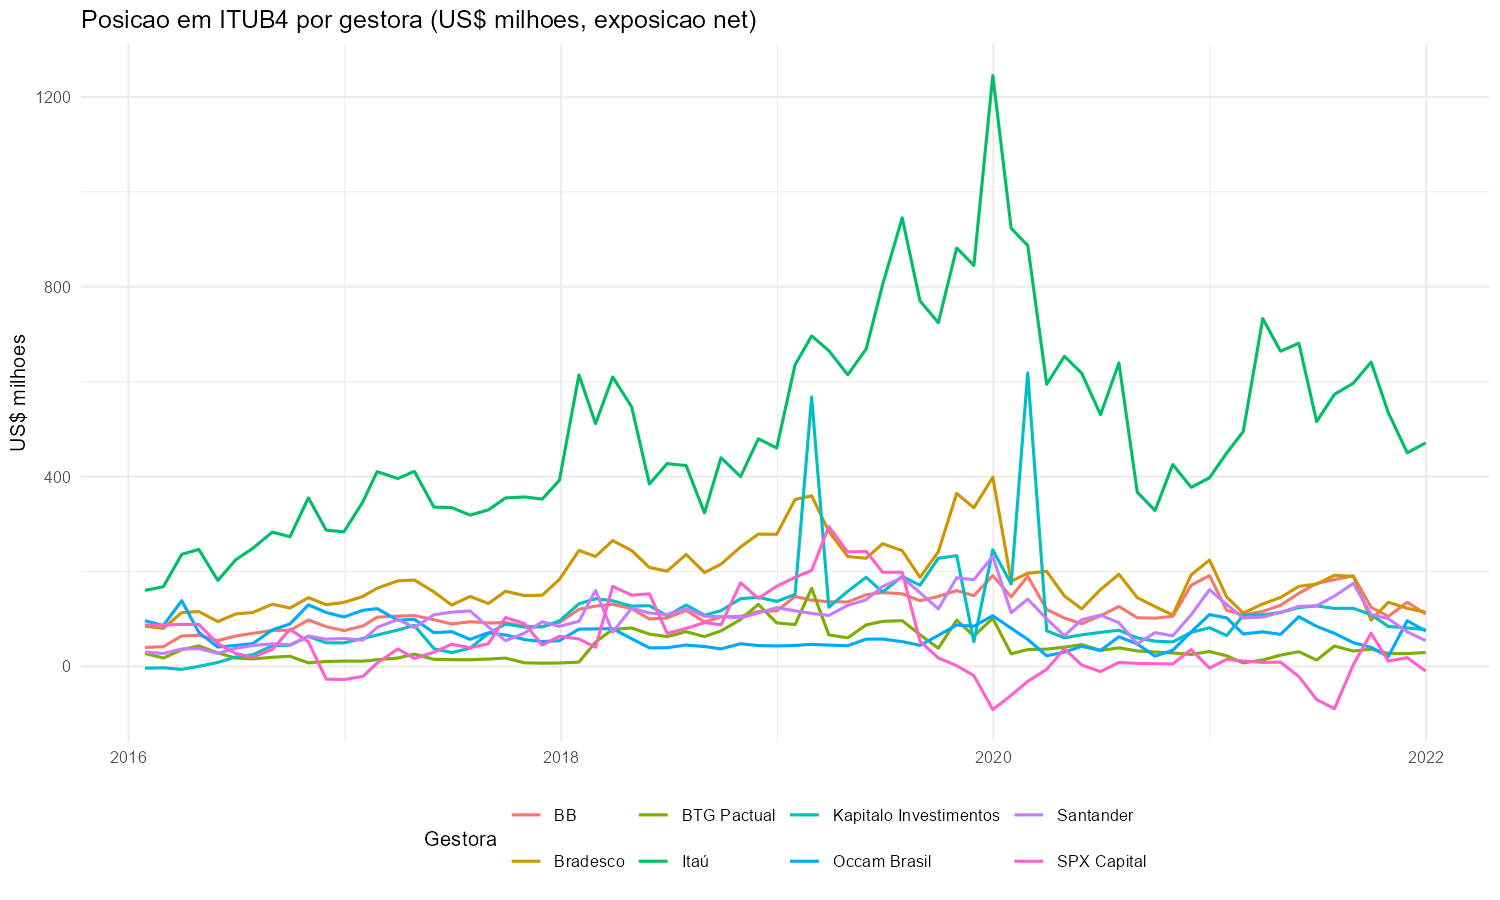
\includegraphics[width=0.88\textwidth]{pos_usd_top_gestoras.png}
\caption{Posição em ITUB4 por gestora (US\$ milhões, net).}
\label{fig:pos}
\end{figure}

\section{Extensão exploratória: o grafo fundo-sobre-fundo}\label{sec:grafo}
Como extensão ao painel CONS+SH, reconstruímos um grafo direcionado a partir da CDA Bloco~2
(\texttt{igraph}). Em \textbf{nenhum} dos 72 meses há estrutura circular no subgrafo observado (sempre
acíclico), mas o \textbf{aninhamento é profundo}: a cadeia mais longa tem mediana 7 e máximo 9 níveis. O
resultado exploratório principal é a \textbf{dupla contagem interna}: a exposição bruta de ITUB4
(R\$\,496 bi) cai para R\$\,310 bi de-duplicada --- \textbf{37,6\%} de duplicação dentro da mesma gestora;
para a Itaú, 41,7\% (Figura~\ref{fig:dedup}). Se, em vez da unidade ``gestora'', a pergunta for a duplicação
rastreável no sistema observado, as arestas entre gestoras adicionam cerca de 5,3 p.p. para ITUB4
(43,0\% no total in-universe). Essa distinção é importante: o número de 37,6\% deve ser lido como duplicação
\emph{intra-gestora}, não como duplicação total do sistema.

\begin{figure}[H]\centering
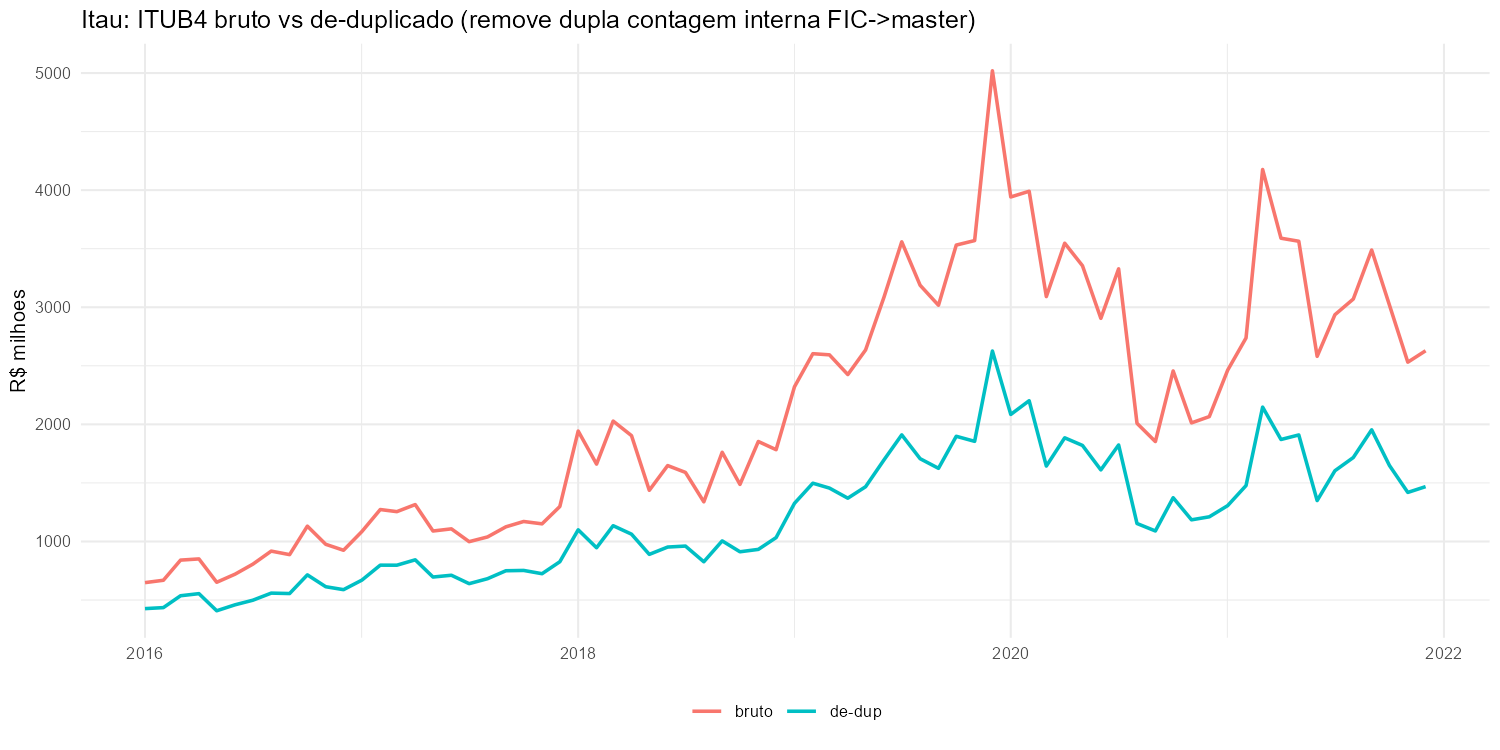
\includegraphics[width=0.85\textwidth]{itub4_dedup_itau.png}
\caption{Itaú: ITUB4 bruta vs de-duplicada (remove a dupla contagem interna FIC$\to$master).}
\label{fig:dedup}
\end{figure}

\section{Generalização e concentração}\label{sec:geral}
Estendendo a \textbf{836 ações}, o painel principal mostra que as ações detidas por \textbf{todas} as 42
gestoras são as \emph{blue chips} (VALE3, PETR4, ITUB4, BBDC4, EQTL3\ldots), exatamente as mais frágeis no
sentido de \citet{greenwoodthesmar2011} (Figura~\ref{fig:crowd}). No módulo complementar com CDA, a exposição
total em ações cai de R\$\,14,3 tri (bruta) para R\$\,8,9 tri (de-dup), \textbf{37,4\%} de duplicação
intra-gestora --- praticamente igual ao ITUB4 --- e o número se repete ação a ação (a maioria entre 30\% e
42\%). Esse resultado é substantivo, mas depende da aceitação da CDA como extensão metodológica.

\begin{figure}[H]\centering
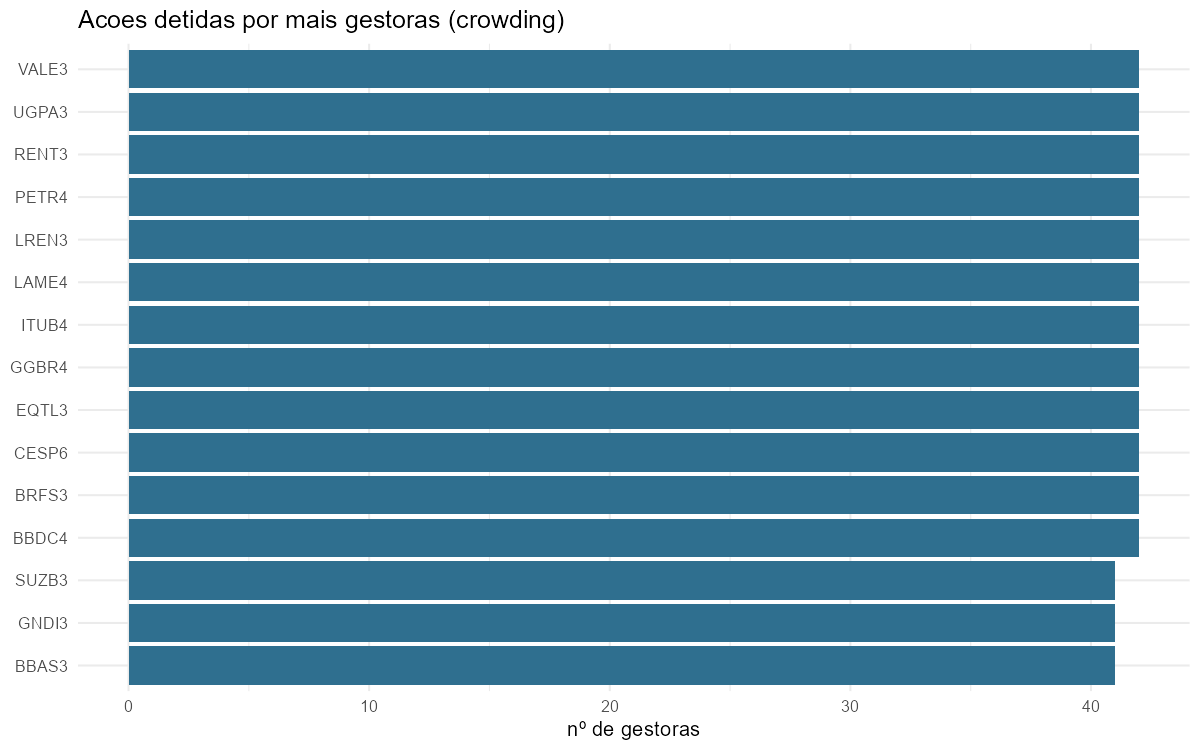
\includegraphics[width=0.8\textwidth]{stock_crowding_top15.png}
\caption{Ações detidas pelo maior número de gestoras (\emph{crowding}).}
\label{fig:crowd}
\end{figure}

\section{Previsibilidade da exposição}\label{sec:fc}
Cinco rodadas \emph{out-of-sample} (Tabela~\ref{tab:fc}): a \textbf{variação} mensal da posição é
\textbf{imprevisível} (nenhum modelo bate o RW; direção 50,8\%, cara-ou-coroa). Mudando o alvo para o
\textbf{nível}, surge previsibilidade por \textbf{reversão à média} (AR bate o RW em $\sim$10\% para ITUB4).
Em uma especificação complementar que usa a rede da CDA, \textbf{features de rede} não acrescentam
($\gamma\approx0$) --- um GNN seria improvável de ajudar a \emph{prever}. Ao generalizar para 238 ações, a previsibilidade \textbf{não é geral}: concentra-se nas
\emph{blue chips} (ITUB4 entre as 3 mais previsíveis; mediana $-13{,}5\%$, Figura~\ref{fig:fc}).

\begin{table}[H]\centering
\caption{Previsibilidade da exposição (\emph{skill} vs random walk).}
\label{tab:fc}
\small
\begin{tabular}{ll}
\toprule
\textbf{Alvo / pergunta} & \textbf{Resultado} \\
\midrule
Variação mensal ($\Delta$ posição US\$) & imprevisível; RW imbatível; direção 50,8\% \\
Nível da posição (ITUB4)         & previsível: AR $+\sim$10\% vs RW (reversão à média) \\
Peso                             & $\approx$ random walk \\
Features de rede (vizinhos)      & não acrescentam ($\gamma\approx0$) \\
Generalização (238 ações)        & só nas \emph{blue chips} (ITUB4 top-3; mediana $-13{,}5\%$) \\
\bottomrule
\end{tabular}
\end{table}

\begin{figure}[H]\centering
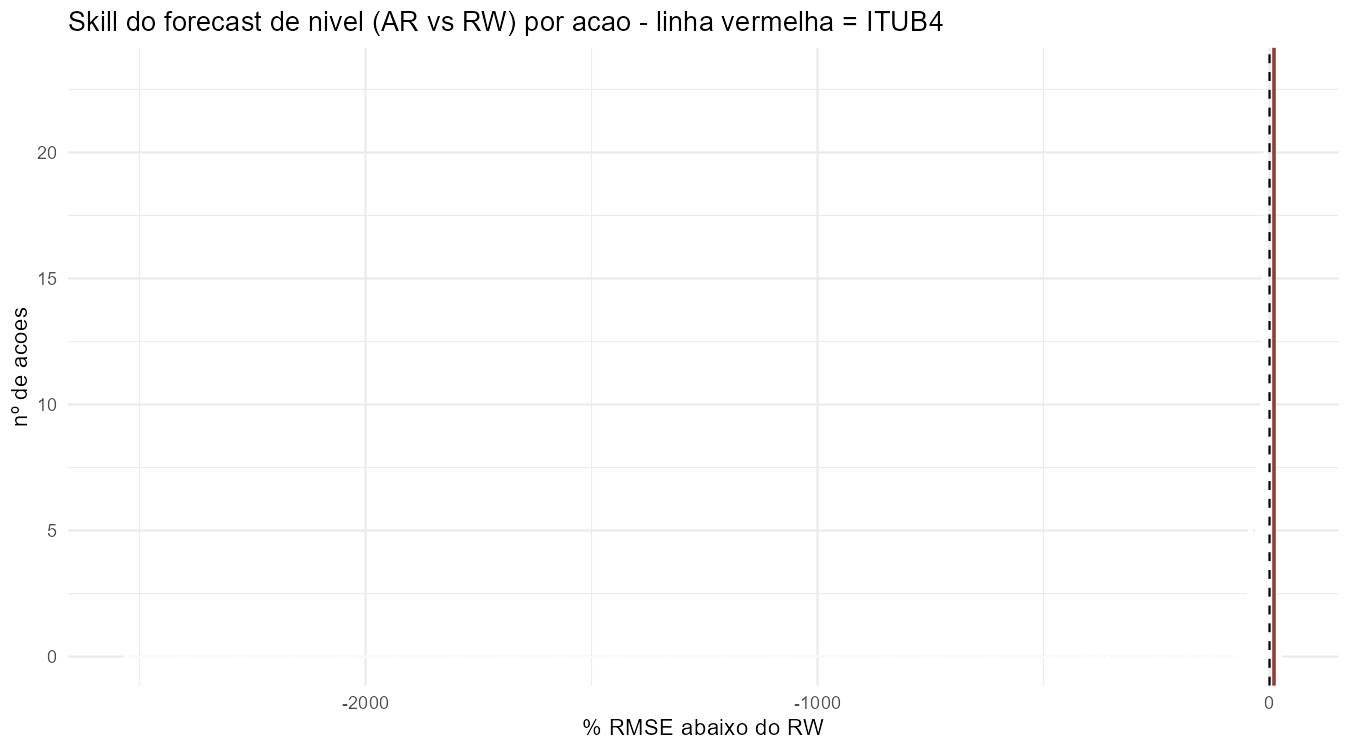
\includegraphics[width=0.82\textwidth]{forecast_round5_skill_hist.png}
\caption{\emph{Skill} do forecast de nível por ação (238 ações). Linha vermelha $=$ ITUB4.}
\label{fig:fc}
\end{figure}

% =================================================================
\chapter{Discussão e conclusão}\label{cap:disc}
Os resultados formam um quadro coerente. \textbf{Medição:} com CONS+SH, o projeto entrega um painel
reprodutível de exposição institucional em valor. \textbf{Previsão:} a demanda muda de forma quase
imprevisível no curto prazo; o componente previsível é a reversão a uma \emph{alocação-alvo}, concentrada
justamente nos papéis mais \emph{crowded}. \textbf{Extensão CDA:} ao reconstruir relações fundo$\to$fundo, a
CDA sugere que somas ingênuas de fundos da mesma gestora podem superestimar a exposição por dupla contagem
interna em torno de 37\%. Essa é uma evidência relevante para o eixo de risco, mas deve permanecer como
resultado complementar até validação explícita do uso da CDA no desenho do TCC.

\paragraph{Limitações.} Painel curto (72 meses) e frequência mensal; validação centrada nas \emph{blue chips};
na CDA, parte relevante das arestas aponta para fundos externos ao universo e o campo de confidencialidade
exige leitura cuidadosa, pois nos históricos processados o CNPJ do fundo investido aparece preenchido mesmo
quando \texttt{DT\_CONFID\_APLIC} existe. \textbf{Próximos passos:} confirmar com o orientador se a CDA deve
ficar no corpo do TCC ou apenas em apêndice; incorporar a meia-vida da reversão; aprofundar métricas de risco
da rede somente se esse eixo for aprovado.
Todo o \emph{pipeline} (R) é reprodutível e versionado.

\bibliographystyle{plainnat}
\bibliography{refs}
\end{document}
